\section{variación de los grados de Polinomios}


\begin{figure}[h]
    \centering
    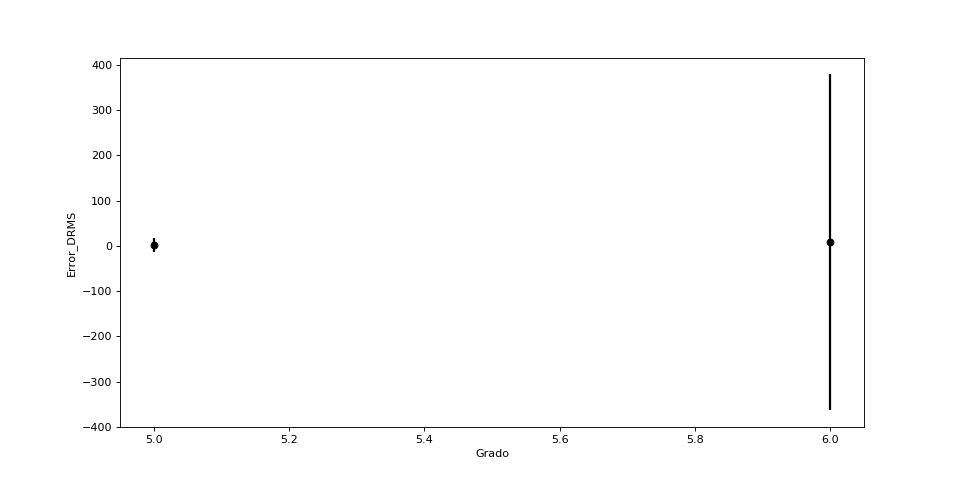
\includegraphics[width=\textwidth]{1_6.png}
    \caption{}
    \label{}
\end{figure}
\begin{figure}[h]
    \centering
    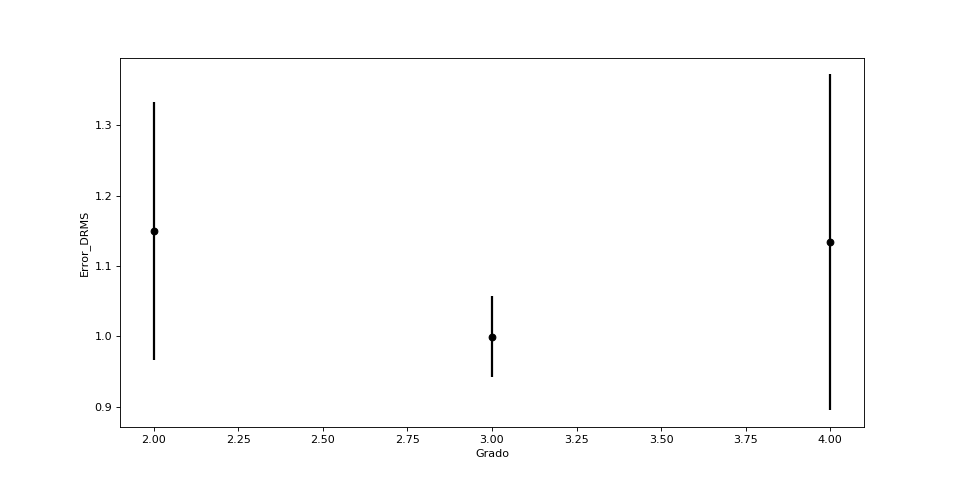
\includegraphics[width=\textwidth]{2_4.png}
    \caption{}
    \label{}
\end{figure}
\begin{figure}[h]
    \centering
    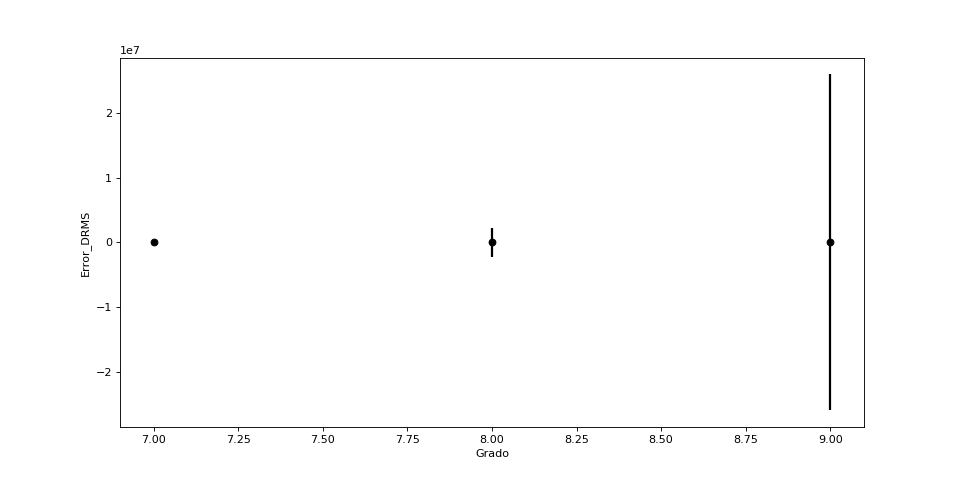
\includegraphics[width=\textwidth]{2_9.png}
    \caption{}
    \label{}
\end{figure}

\begin{figure}[h]
    \centering
    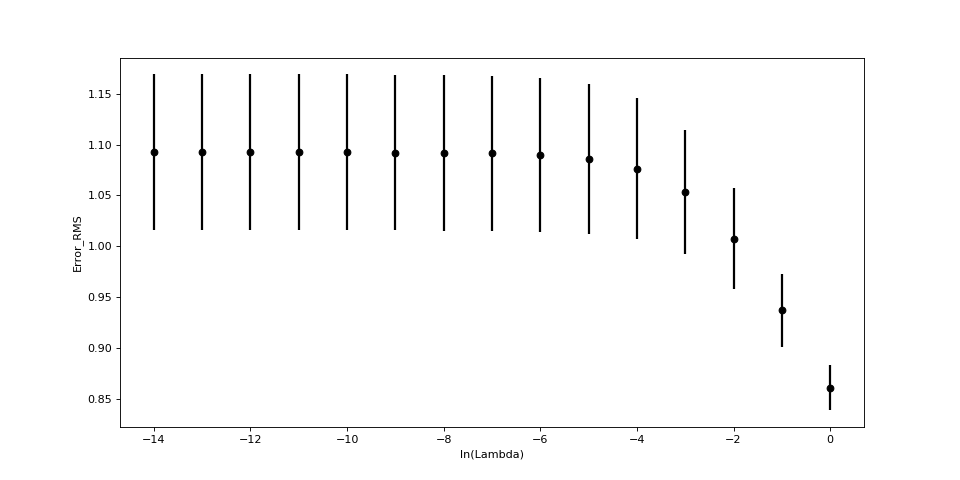
\includegraphics[width=\textwidth]{error_INDUS_lambda.png}
    \caption{}
    \label{error_INDUS_lambda}
\end{figure}
\begin{figure}[h]
    \centering
    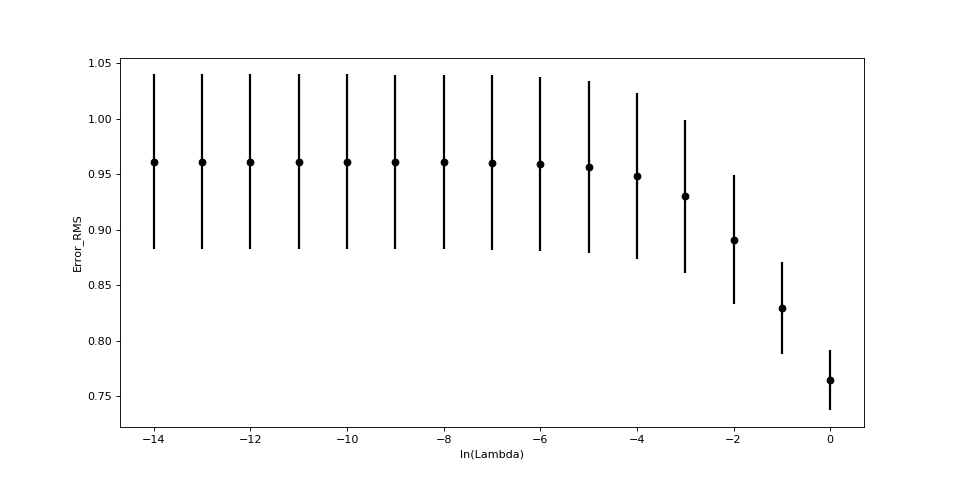
\includegraphics[width=\textwidth]{error_INDUSNOXRMAGETAX_lambda.png}
    \caption{}
    \label{error_INDUSNOXRMAGETAX_lambda}
\end{figure}
\begin{figure}[h]
    \centering
    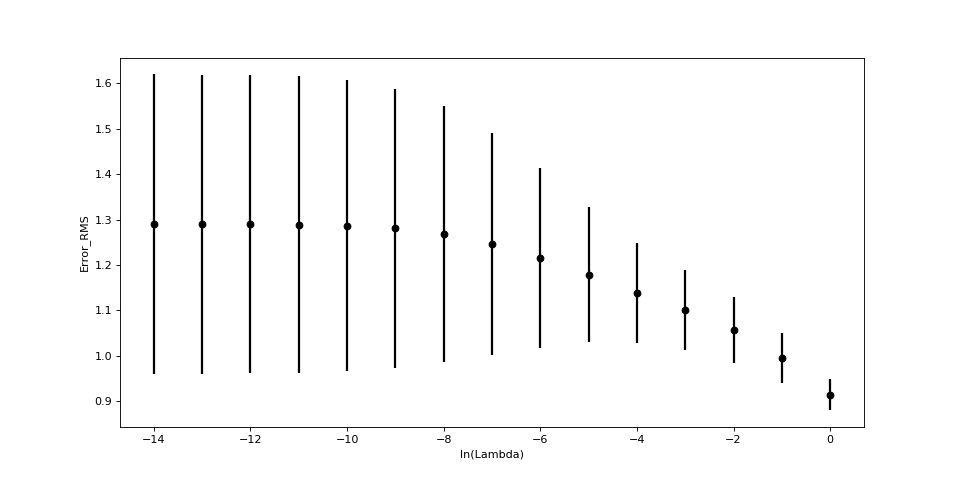
\includegraphics[width=\textwidth]{error_NOX_lambda.png}
    \caption{}
    \label{error_NOX_lambda}
\end{figure}




\begin{figure}[h]
    \centering
    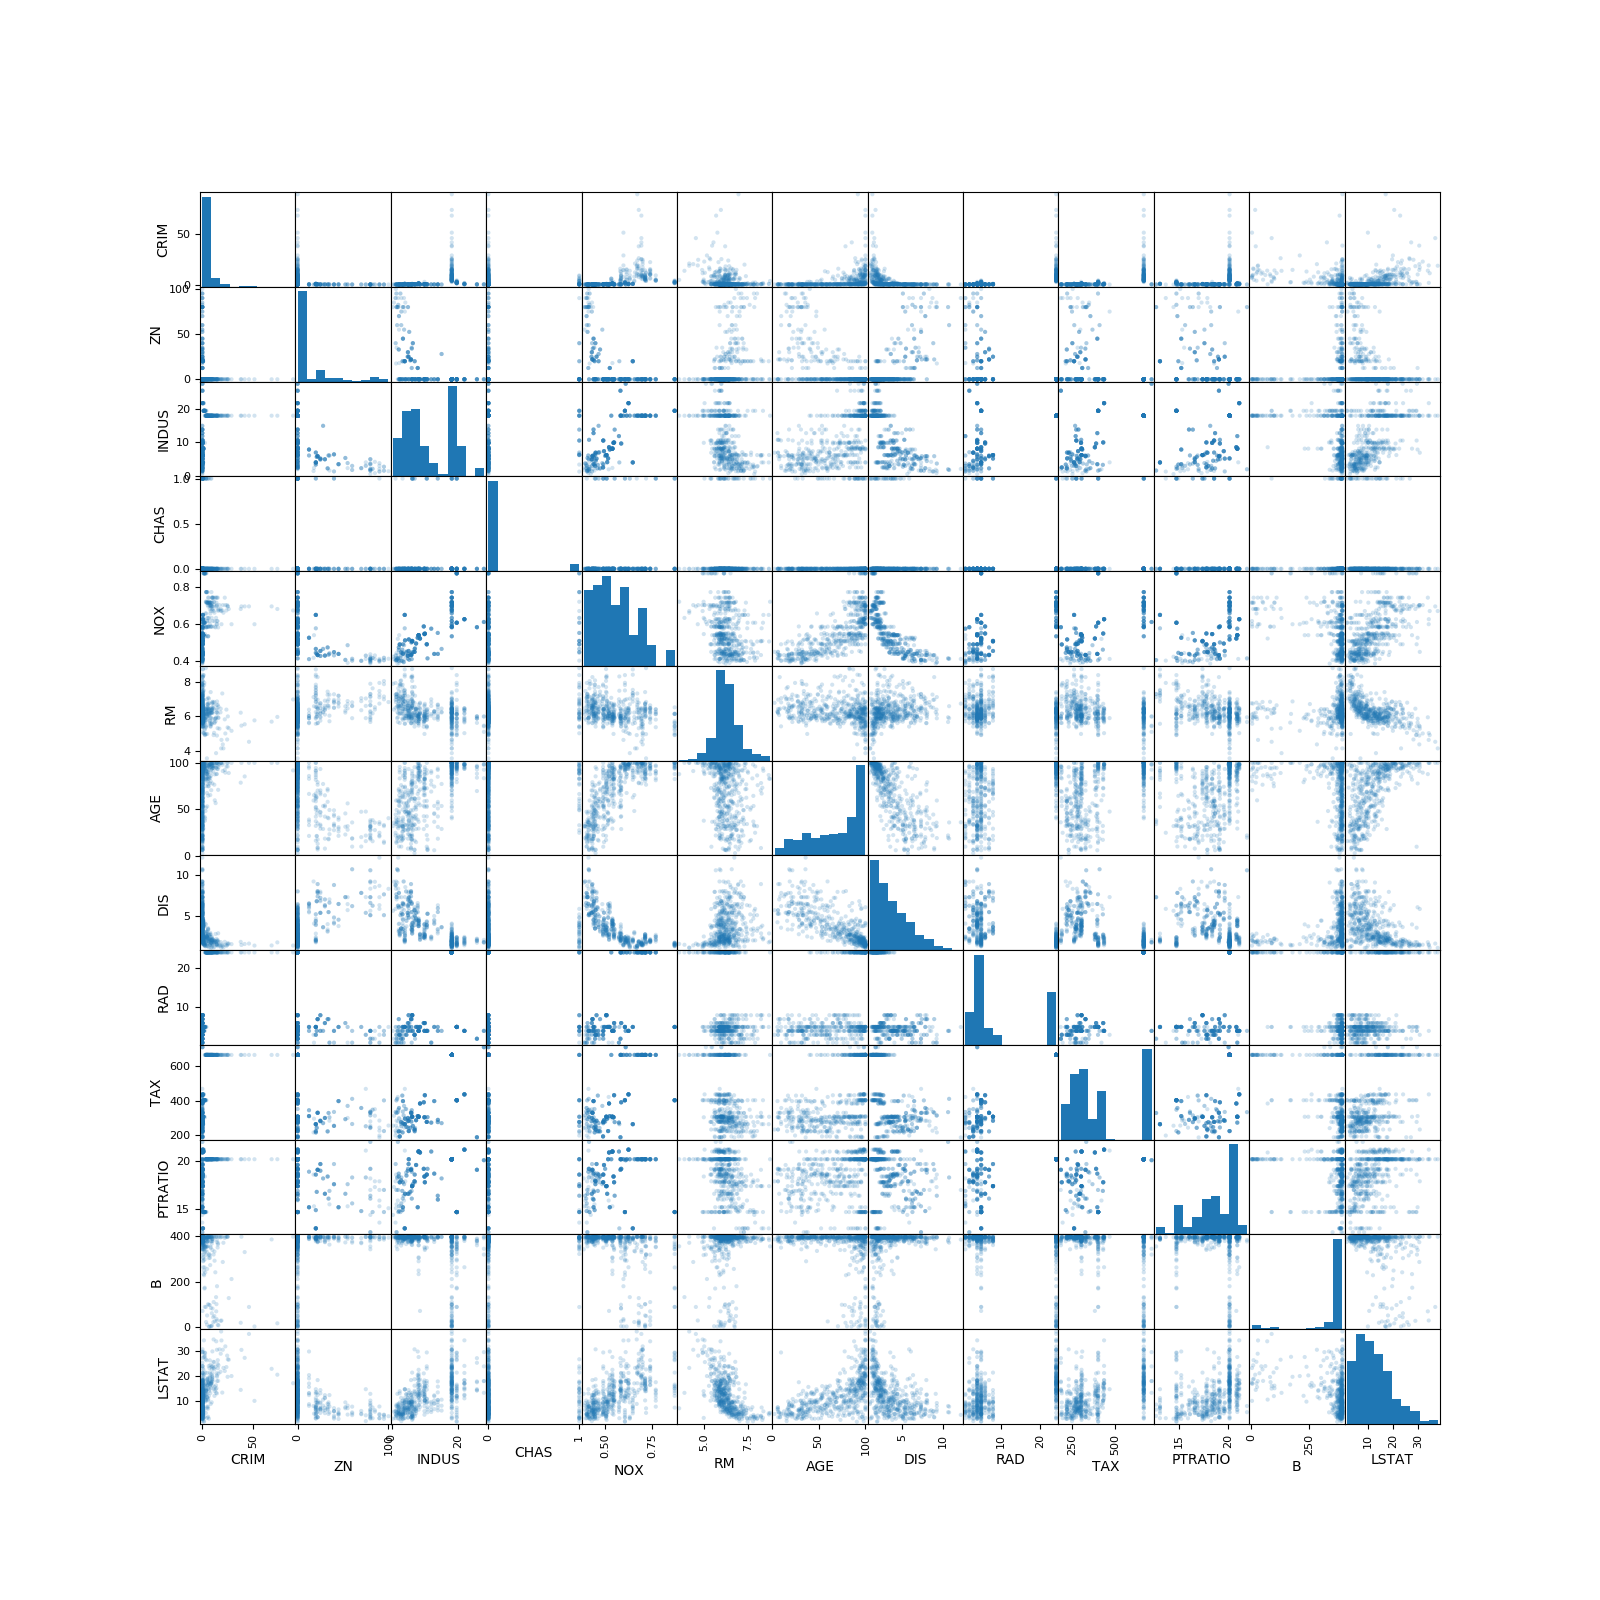
\includegraphics[width=\textwidth]{scatter.png}
    \caption{Scatter-plots de Boston Housing Dataset}
    \label{scatter}
\end{figure}
\begin{figure}[h]
    \centering
    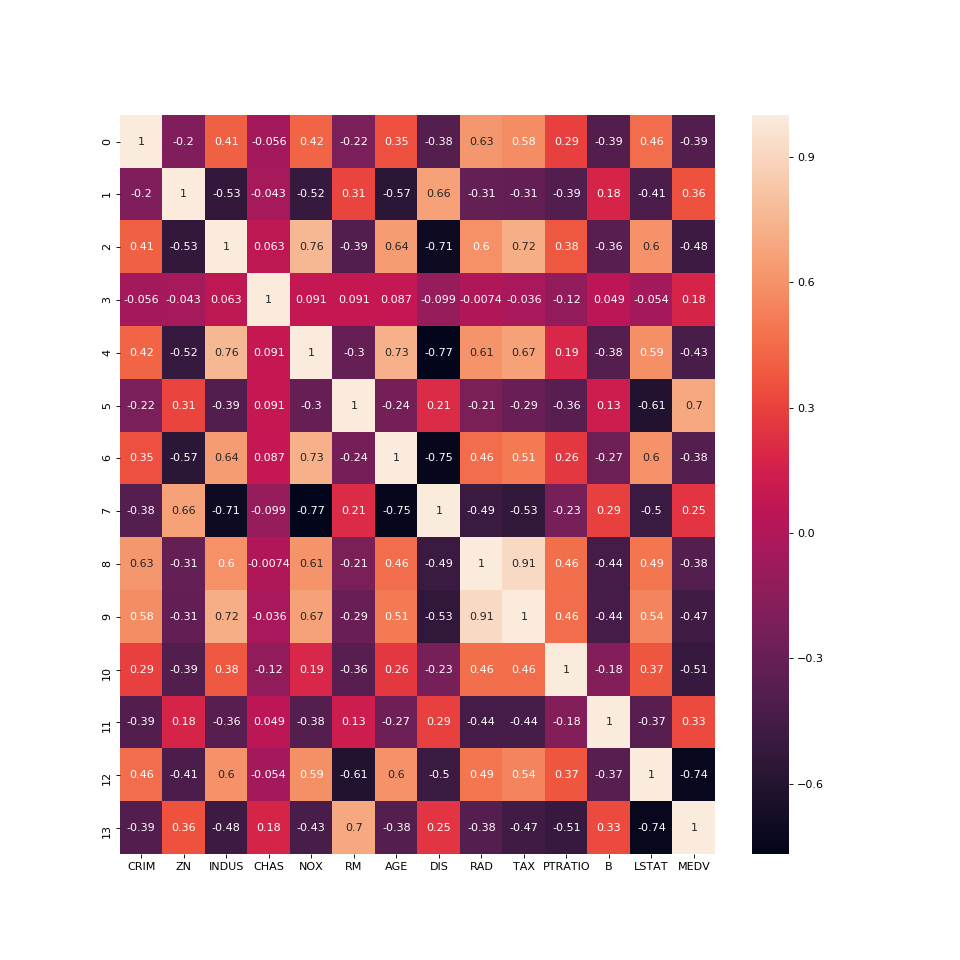
\includegraphics[width=\textwidth]{matriz_correlacion.png}
    \caption{Matriz de correlación de Boston Housing Dataset}
    \label{matriz_correlacion}
\end{figure}
\begin{figure}[h]
    \centering
    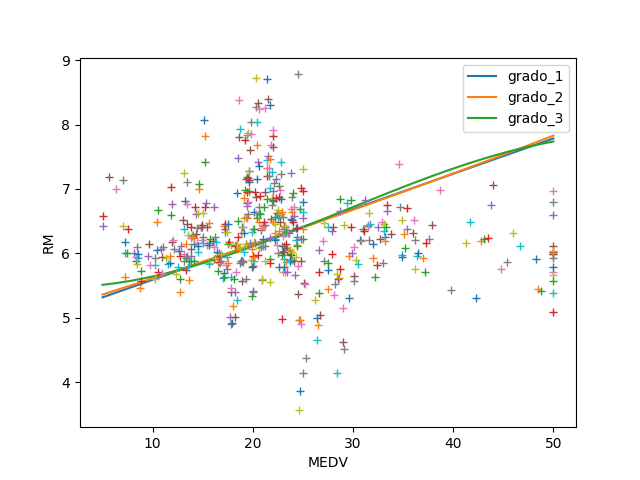
\includegraphics[width=\textwidth]{rmXmedv.png}
    \caption{Estimación de la distribución de puntos entre MEDV y RM}
    \label{rmXmedv}
\end{figure}
\begin{figure}[h]
    \centering
    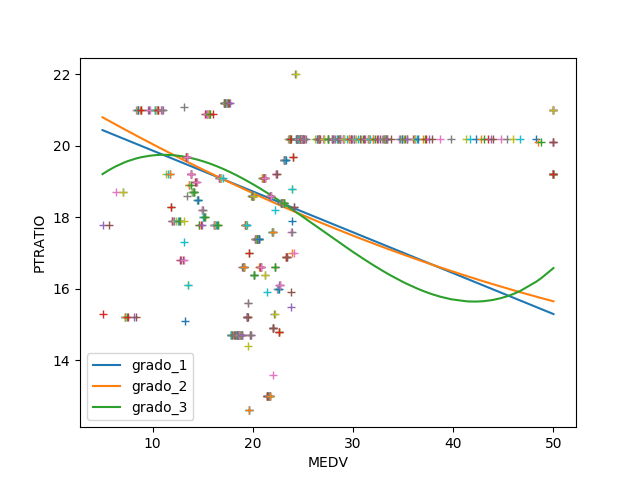
\includegraphics[width=\textwidth]{ptratioXmedv.png}
    \caption{Estimación de la distribución de puntos entre MEDV y PTRATIO}
    \label{ptratioXmedv}
\end{figure}
\begin{figure}[h]
    \centering
    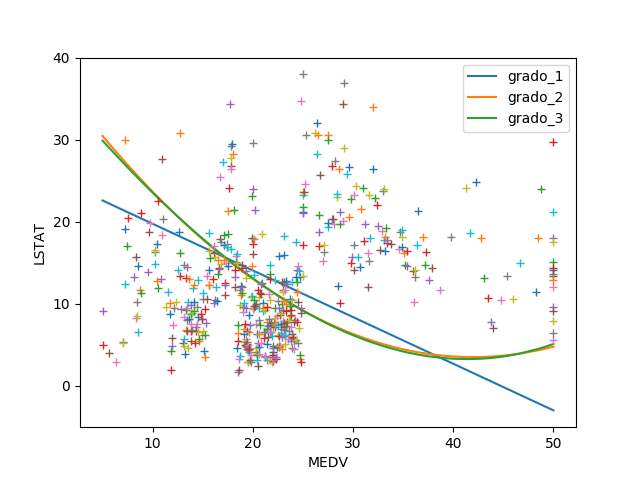
\includegraphics[width=\textwidth]{lstatXmedv.png}
    \caption{Estimación de la distribución de puntos entre MEDV y LSTAT}
    \label{lstatXmedv}
\end{figure}
\begin{figure}[h]
    \centering
    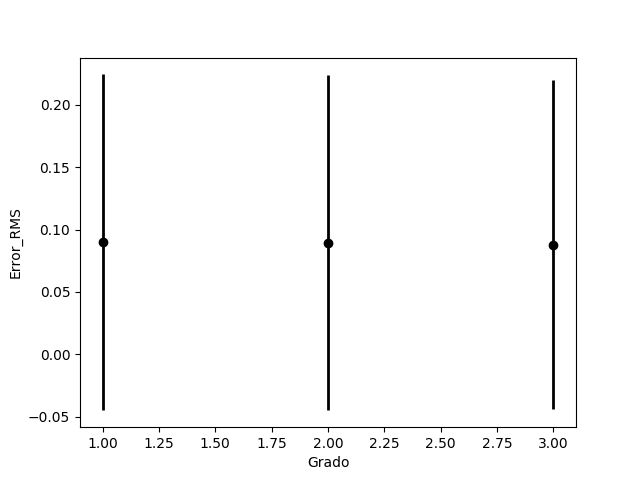
\includegraphics[width=\textwidth]{errorRM.png}
    \caption{Media y Varianza al estimar la relación entre MEDV y RM}
    \label{errorRM}
\end{figure}
\begin{figure}[h]
    \centering
    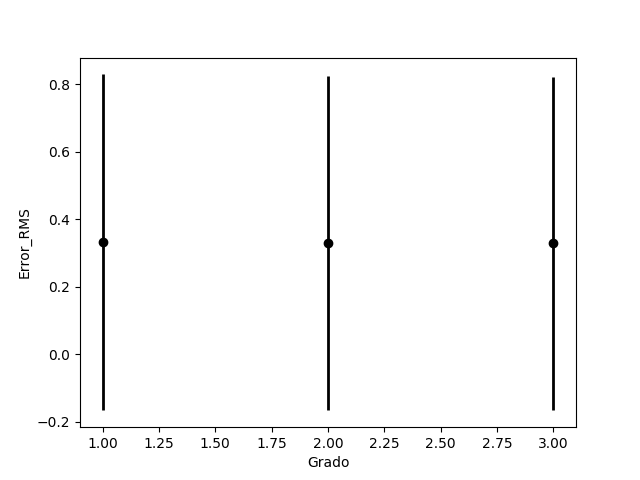
\includegraphics[width=\textwidth]{errorPTRATIO.png}
    \caption{Media y Varianza al estimar la relación entre MEDV y PTRATIO}
    \label{errorPTRATIO}
\end{figure}
\begin{figure}[h]
    \centering
    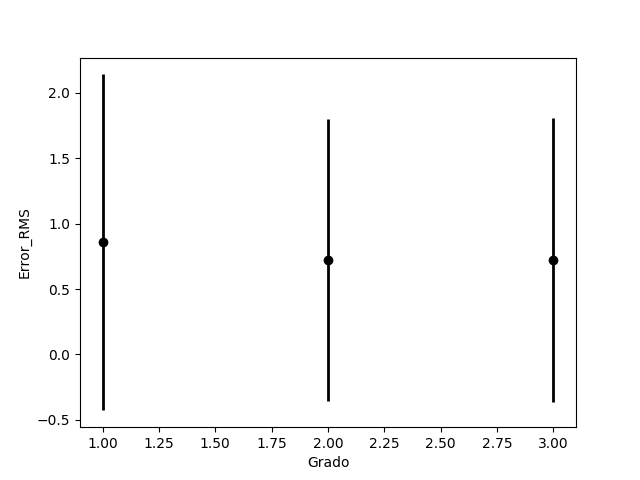
\includegraphics[width=\textwidth]{errorLSTAT.png}
    \caption{Media y Varianza al estimar la relación entre MEDV y LSTAT}
    \label{errorLSTAT}
\end{figure}